% Chapter 2

\chapter{Deep Neural Networks and Parallelism} % Main chapter title

\label{Chapter2} % For referencing the chapter elsewhere, use \ref{Chapter2} 

%----------------------------------------------------------------------------------------
\section{Deep Learning Applications}

Deep learning and the progress made in that field have all fueled its integration into many applications of daily life \cite{ddl}. In the early days, the results of machine learning were dependent on the quality and informativeness of the features fed into the learning algorithm \cite{csaji2001approximation}. With the development of deep neural nets, the machine itself can abstract raw data and learn complex features that become much more informative than the hand-engineered ones \cite{lecun2015deep}. Modern architectures are able to process and incoming stream of images, video, or speech and learn to classify those raw data and solve complex problems in image segmentation and speech recognition \cite{lecun2015deep, resnet, densenet}. What is also important is that the value gained by those architectures increases as more data and more computational resources are presented to the network for training. Learning can be supervised, semi-supervised, and unsupervised \cite{lecun2015deep}. Supervised learning is a problem of finding the best mapping between a set of input data $\mathit{X}$ and a set of output labels or values $\mathit{Y}$ \cite{lecun2015deep}. Learning algorithms proceed in approximating the mapping function $\mathit{ f : X \rightarrow Y}$ by observing both the inputs and the labels. Learning stops when an acceptable approximation of $\mathit{f}$ is found. Supervised learning can be split into two categories; classification when the output variable is a given label as in objects : \emph{"table"} , \emph{“penguin”} , or \emph{“motorcycle”}, and regression when the output variable is a real-value such as \emph{"temperature"} or \emph{"dollar value"}. The goal of unsupervised learning on the other hand is to discover a data model or structure of the given data. There are no given labels or output variables and the goals is to learn something useful about the data. Unsupervised learning is split also into two categories; clustering by splitting the data into groups having similar attributes, and association where we want to discover rules that describe a large subset of the observed data ( ex. People who work at \emph{"X"} tend to buy product \emph{"Y"} ). Semi-supervised learning is situated somewhere in between supervised and unsupervised learning where only a subset of the data is labeled. Solving these problems requires both supervised techniques to label the unlabeled data and feed back in the labels for training, or the data can be used to uncover structure. Our work focuses more on supervised learning as the majority of deployed applications use supervised learning. We attempt to accelerate the training process of deep neural networks on FPGAs. 

%----------------------------------------------------------------------------------------
\section{Convolutional Neural Networks}

Convolutional Neural Networks have achieved many successes in multidimensional data than can be represented as arrays \cite{lenet, alexnet, resnet}. A typical image can be represented as a three-channeled ( Red, Green, and Blue ) two-dimensional array of varying pixel intensities. A convolutional neural net is mainly composed of two stages that make sense of structured grid-like data to accomplish a learning task such as classification, regression, or even dimensionality reduction. An initial stage of convolution operators that pass a window filter over the image to extract an output feature map as in a discrete convolution operator. The convolution operation was inspired by a cat’s visual cortex and how neurons in the brain are triggered by certain shapes like lines in the seen image \cite{hubel1962receptive}. The intuition behind the convolution operation as a feature extraction method is that nearby pixels exhibit similarities and show high correlations \cite{lavin2016fast}. Also the image patches extracted in the convolution windows which represent concepts can appear anywhere elsewhere in the image. The convolution layers are usually followed by non-linear activations and then pooling operators. The role of pooling layers is to merge the similar nearby features into one to decrease the sensitivity of the network to the position of the extracted feature \cite{szegedy2015going}. The second stage of a CNN is a series of fully connected layers ultimately terminating at an output layer.

\subsection{Case Study : LeNet-5}
The LeNet \cite{lenet} model is considered to be the first demonstration of a convolutional neural network and was proposed by LeCun et. al \cite{lenet} in 1998. Its architecture has shown record accuracy in classifying digits and was deployed commercially for identifying characters on personal and business checks. LeCunn’s work was the first to demonstrate the benefit of brute-force numerical tricks in convolutions and that these tricks can be more useful than hand-engineering traditional feature engineering techniques \cite{lenet}. Also compared to traditional neural networks, the convolution layers are more robust as the extracted features are shift and translation invariant. This proved to be efficient since handwritten characters differ in slant and scale from one person’s handwriting to another’s and it was hard back then to perform feature preprocessing to documents such as normalization and centering handwritten characters.

\subsubsection{Architecture}

\begin{figure}[h!]
\centering
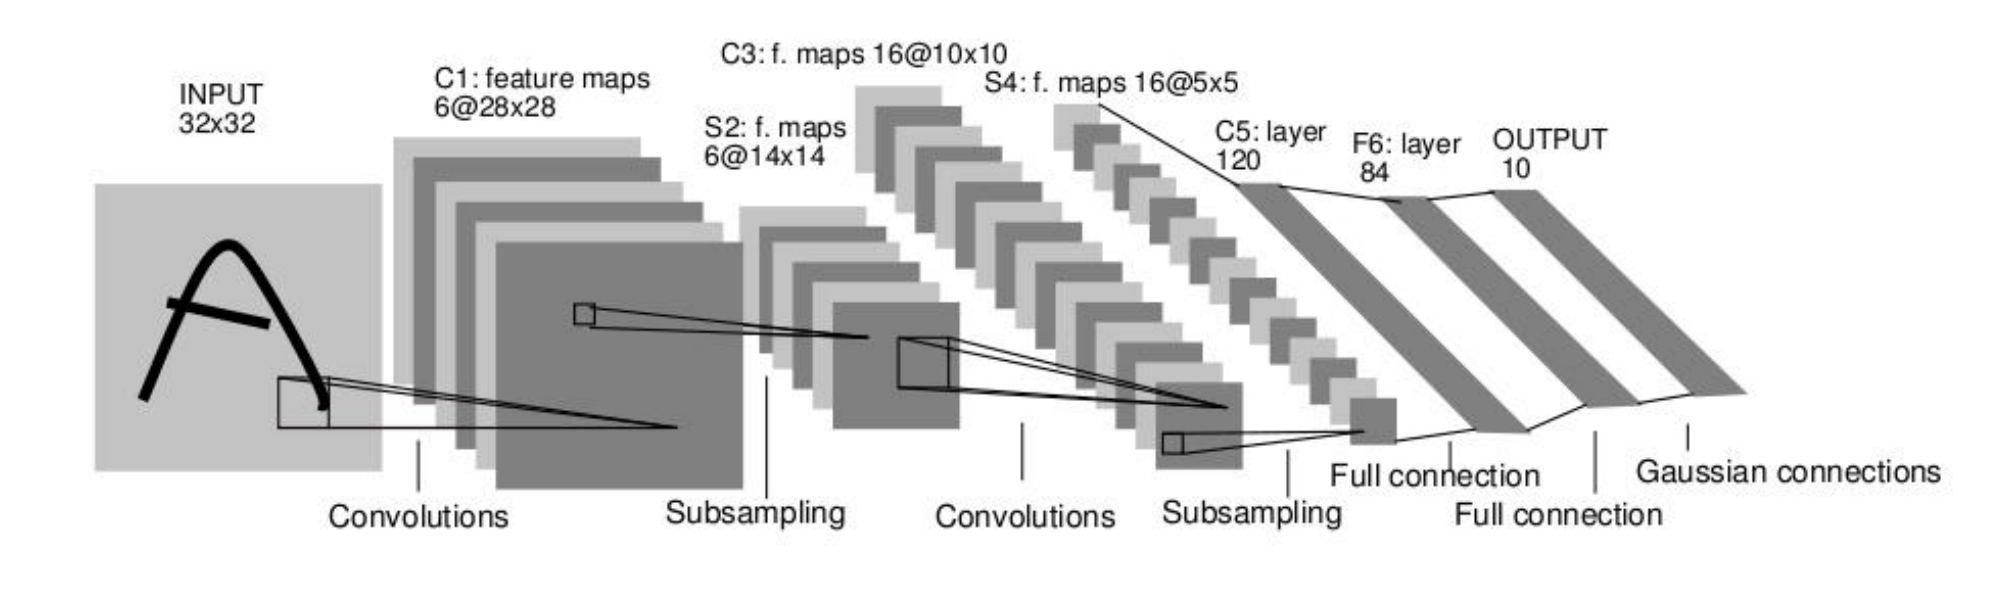
\includegraphics[width=1.0\textwidth]{Figures/lenet}
\decoRule
\caption[LeNet]{ LeNet-5 Architecture, a convolutional neural network used for character recognition. \cite{lenet}}
\label{fig:Lenet-5}
\end{figure}

The Lenet-5 is comprised of 7 layers ( excluding the input layer ), all of which contain trainable parameters. The input is a centered 32x32 image which represents the raw data that is fed into the network. It is followed by a convolutional layer and a subsampling layer. The first convolutional layer C1 produces an output of 6 distinct feature maps. Each feature map is obtained by sliding a 5x5 filter along the input image and computing a weighted sum of the pixels inside the window. This leads to shrinking the image by 4 pixels along both dimensions, and 6 features are obtained by passing 6 different weights for the filters. A bias is added to the weighted sum of pixels and it is squashed by the sigmoid function before feeding into the output feature map. 

The convolutional layer is then followed by a subsampling layer with a window size of 2x2. The four feature maps elements in C1 are added, multiplied by a trainable coefficient and then a trainable bias is added. The six feature maps of C1 are halved in size along both dimensions and the resulting feature maps at S2 are six 14x14 arrays. 

\begin{figure}[h!]
\centering
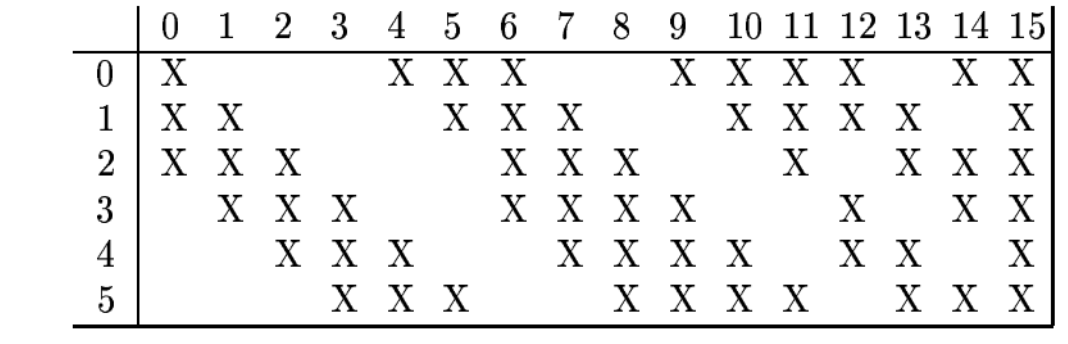
\includegraphics[width=0.65\textwidth]{Figures/connections}
\caption[Connections]{ Each column indicates which feature maps in S2 are combined by the units in a particular feature map of C3. \cite{lenet}}
\label{fig:Lenet Connections}
\end{figure}

Similarly the feature maps at S2 are followed by another convolution and another subsampling layer C3 and S4. The outputs of S2 however are not connected all-to-all to the third convolution instead only the marked slots in the table 1 below shows that only some combinations of the feature maps in S2 are connected to C3. The purpose is to avoid overfitting to the full S2 features by breaking the symmetry and hopefully discovering different feature abstractions from the different set of inputs \cite{lenet}. It also serves to decrease the amount of trainable parameters in the model. 

The convolution stage ( C1  $\rightarrow$ S4 ) is followed by two fully connected layers C5 and F6 of sizes 120 and 84 neurons respectively. Note that the reason C5 is labeled as a convolution layer (even though it performs the role of a fully connected layer) is that if the network were scaled for bigger inputs, the output feature map for C5 would be larger than 1x1. 

The last fully connected layer is fed into the output which is composed of Euclidean Radial Basis (RBF) \cite{chen1991orthogonal}. It computes the euclidean distance between the input vector and a trainable parameter vector. The model was trained on a set of 60,000 images and achieved a minimum test-error of 0.7\% competing with all of the other neural network models at the time. Some of the input training images were translated slightly, and rotated by up to $\pm{30^\circ}$ to increase the network’s robustness by making it slightly more translation and rotation invariant. 

Even though the Lenet is outdated and has been replaced by many other neural networks, we choose to this network as a prototype to build our DNN framework due to the simplicity of the implementation. We implement it not for its usefulness but rather more to guide our study into optimizing layer implementations and thinking about methods to improve throughput and achieve pipelining between the layers. 

\subsection{Modern Architectures} 

\subsubsection{AlexNet}

\begin{figure}[h!]
\centering
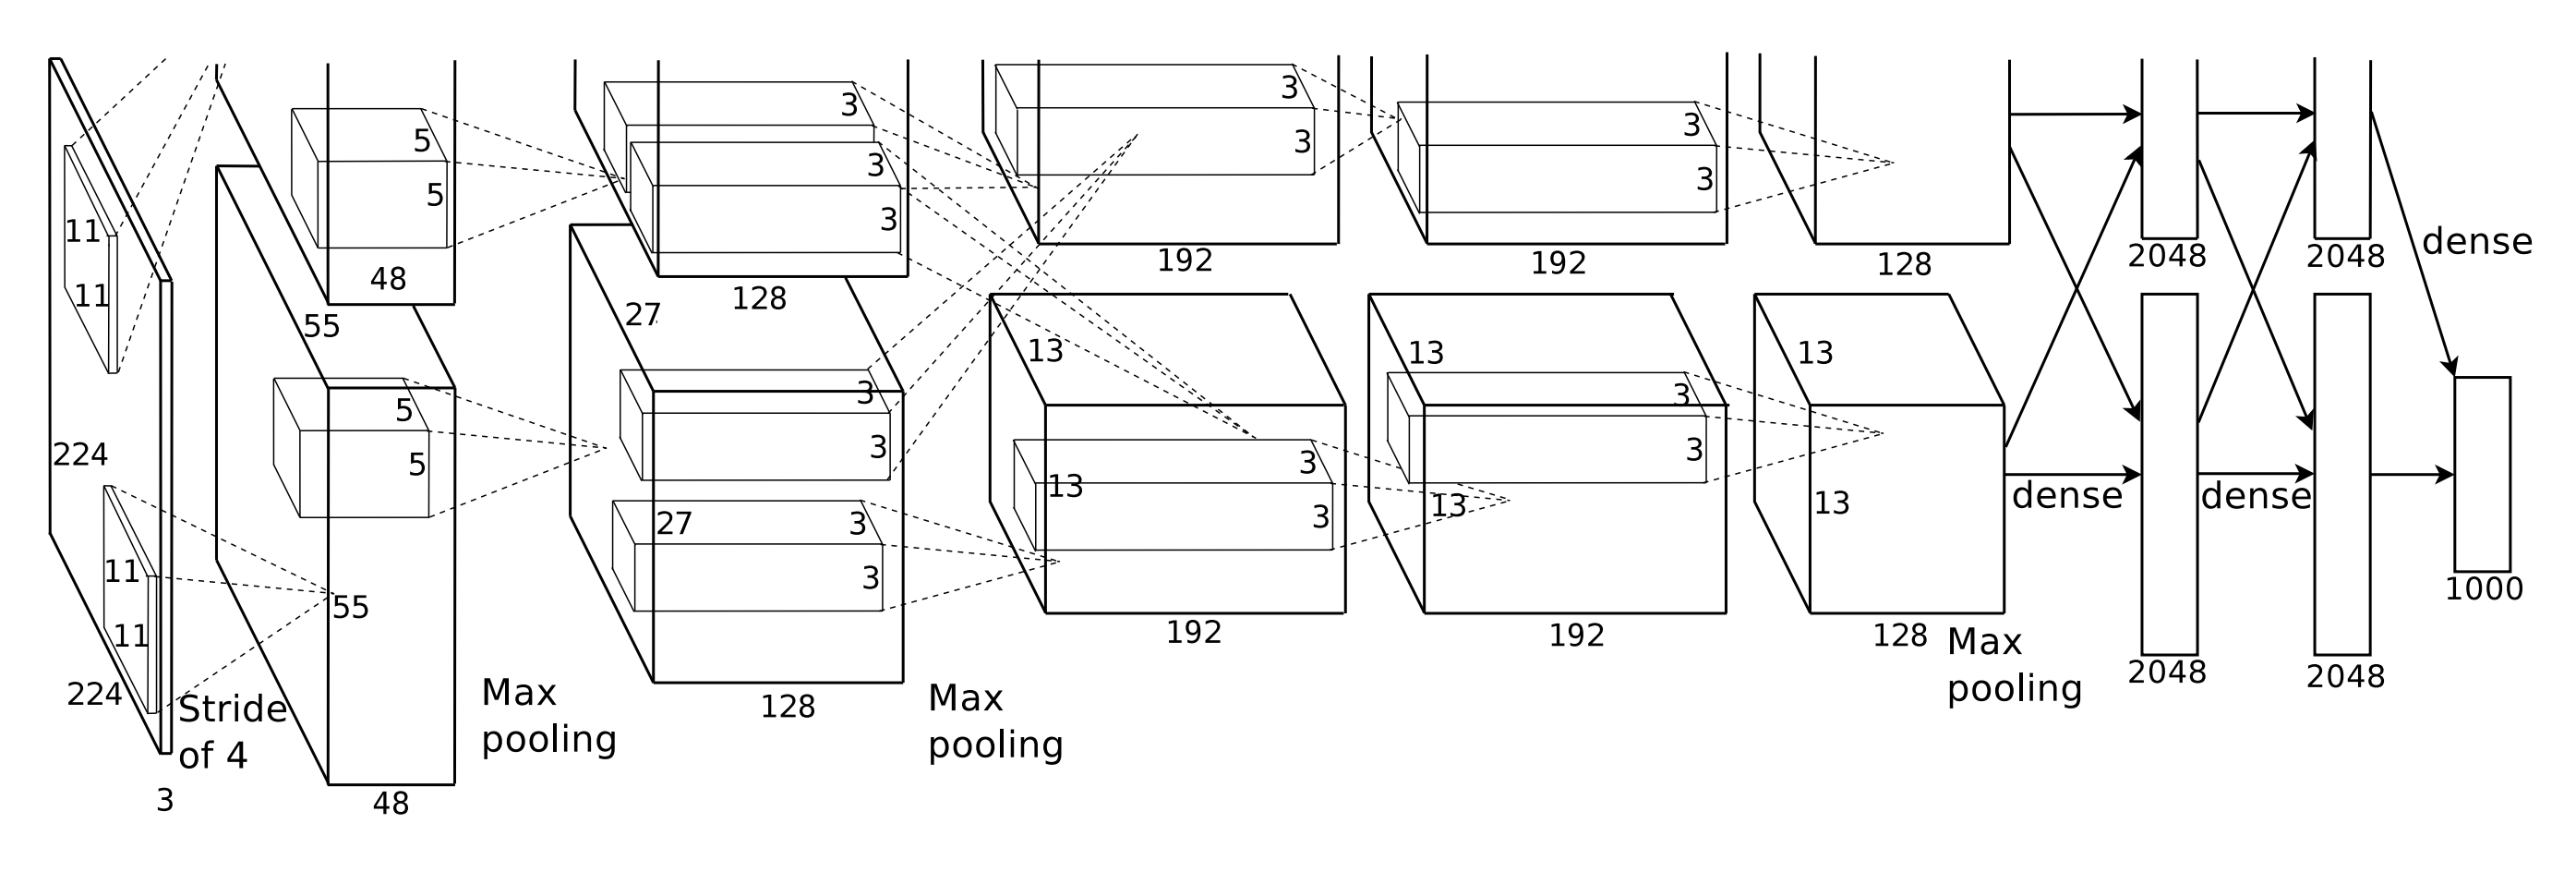
\includegraphics[width=1.0\textwidth]{Figures/alexnet}
\caption[AlexNet]{ Alexnet Architecture  \cite{alexnet}}
\label{fig:AlexNet Architecture}
\end{figure}

The AlexNet \cite{alexnet} model designers won the ImageNet Large-scale Image recognition competition in 2012. It follows LeNet’s approach of staging some convolutional layers back-to-back and then eventually terminating with fully connected layers to perform the classification. It was able to achieve 26.25 top-5 error in the task of classification of three-channeled 224x224 images into 1000 classes. The network was trained on a GPU \cite{alexnet} and used local response normalization layers. In addition to that the authors used dropout which is a technique against overfitting in a network \cite{dropout}. It involves randomly picking out neuron connections and setting them to zero thus decreasing the number of trainable parameters in the model. What also differs from LeNet is the use of Rectified Linear Units (ReLU) activations and maxpooling \cite{alexnet} for the subsampling layers.

\subsubsection{ResNet}

\begin{figure}[h!]
\centering
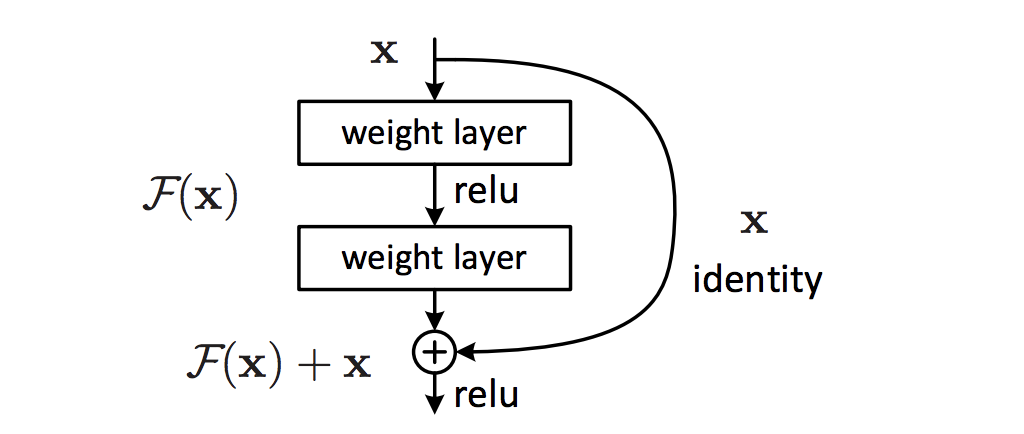
\includegraphics[width=0.7\textwidth]{Figures/residual}
\caption[Residual Learning]{ A basic building block in residual networks showing the identity shortcut  \cite{resnet}}
\label{fig:Residual Learning Basic Block}
\end{figure}

ResNet \cite{resnet} is one of the modern networks that sacrifices breadth for depth. Training deeper network is harder because of a problem discovered by Hochreiter et al. \cite{hochreiter1998vanishing} of vanishing gradients.  The authors of ResNet augment the network with shortcut connections that act as identity layers and enable training with respect to residuals instead of the original input values. Using this trick it was possible to train deeper networks reaching up to more than 150 layers \cite{resnet}. 

%----------------------------------------------------------------------------------------
\section{Training and Backpropagation}  \label{graddesc}

The above networks all try to achieve the goal of properly approximating a mapping function between the dataset inputs and the given labels. In the example of Lenet, inputs are normalized 28x28 single channels, and the output of the network is a the most probable digit between 0 and 9 that this image represents. Formally described, given an input domain $\mathit{X}$, an output set of labels $\mathit{Y}$, and a set of candidate functions $\mathit{f : X \rightarrow Y}$ belonging to a hypothesis class $\mathit{H}$, we are trying to minimize the loss of mispredicting the correct class. The loss function can be expressed as :
\begin{equation}
L_D(f) = p( f(z) \neq h(z)) 
\end{equation} 
 
 where $\mathit{z}$ is a sample from the dataset $\mathit{D}$,  $\mathit{f(z)}$ is the output prediction and $\mathit{h(z)}$ is the true class or label. In that case training is then formalized as finding the best set of parameters $\mathit{w}$ in our model to minimize this loss function. 
\begin{equation}
 w* = \argmin\limits_{ w \in \mathit{H} } L_D(f_w)
 \end{equation}

Several options exists for sample loss functions as shown in Table \ref{tab:loss}. In regression, a common loss function is the squared error loss. In classification problems, the binary loss can be used. However, for minimization, the loss function should be both continuous and differentiable. To solve this problem, an alternative cross-entropy loss function is introduced for multi-class classification problems as opposed to the binary loss. The output becomes a probability distribution of the input according to the given possible output classes. The cross entropy loss calculates the difference between the predicted distribution and the true distribution into $\mathit{K}$ classes.

\begin{table}[h!]
	\centering
	\begin{tabular}{| l | c | r |}
		 \hline
	Squared loss 	& $l=(f_{w}(z)-h(z))^{2}$  \\ \hline
	Binary loss 	&  $l=\left\{\begin{array}{cl} 0, & \mbox{if }f_{w}(z)=h(z)\\ 1, & \mbox{if }f_{w}(z) \neq h(z) \end{array}\right.  $ \\ \hline
	Cross-entropy loss (K classes)	& $l=\sum_{i=1}^{K}f_{w}(z_{i})\log(h(z_{i}))$  \\
	 \hline
	\end{tabular}
\caption[Loss Functions]{Examples of loss functions}
\label{tab:loss}
\end{table}

\subsubsection{Gradient Descent}


To solve the minimization problem, we can either use evolutionary algorithms \cite{fonseca1995overview} inspired by natural processes and meta-heuristics or we can resort to the use of iterative approaches. It is more popular in machine learning to use the iterative gradient descent techniques. In gradient descent, starting from an initial set of weights, we calculate the gradient of the loss function with respect to the weights  $  \frac{\partial L}{\partial w}  $ and iteratively adjust the weights in the direction of the gradient to minimize loss.
\begin{equation}
 w^{t} = w^{t-1} +  \eta \frac{\partial L}{\partial w} 
\end{equation}
The error is back-propagated layer by layer from the output to the input layer by utilizing the chain-rule. $\eta $ is the learning rate, which is a tunable hyperparameter for weight updates.
 
 \begin{figure}[h!]
\centering
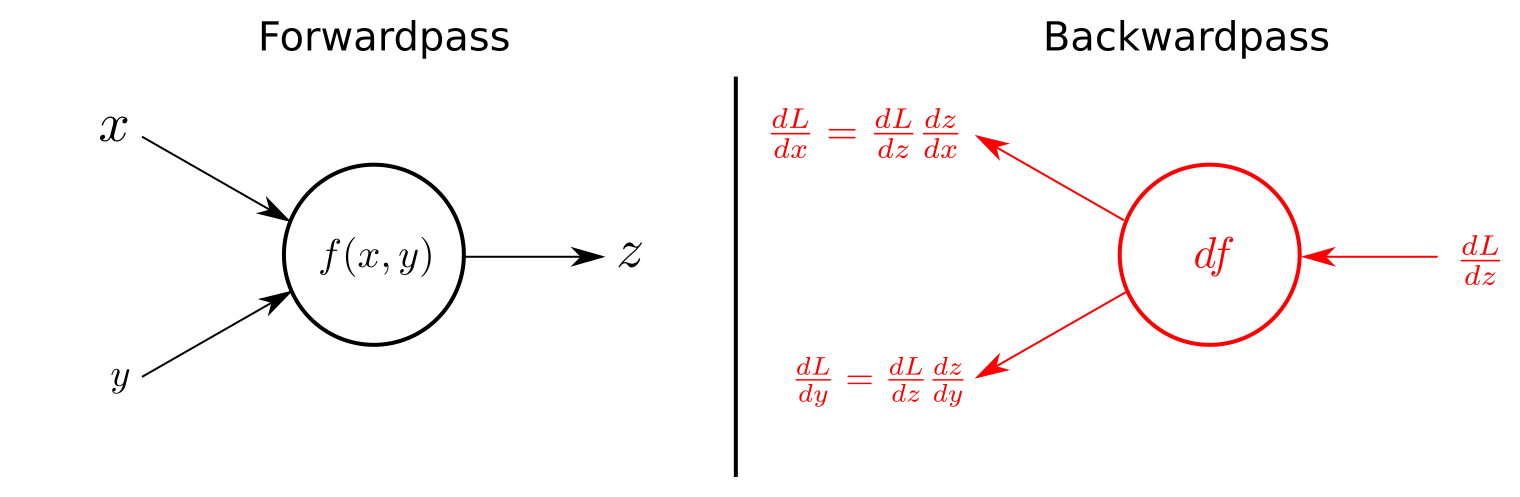
\includegraphics[width=0.9\textwidth]{Figures/backprop}
\caption[Local Backpropagation]{ Local Gradient Backpropagation using the Chain Rule. Source:\footnotemark} 
\label{fig:Forward and Backward Passs}
\end{figure}

\footnotetext{\url{https://kratzert.github.io/2016/02/12/understanding-the-gradient-flow-through-the-batch-normalization-layer.html} Last Accessed: 23/08/2018}
%---Add gradient descent algorithms as pseudo code

%---Compare 3 types of gradient descent
Gradient descent implementations vary depending on how many samples are used to calculate the error. The three main types are batch, stochastic, and mini-batch gradient descent \cite{ruder2016overview}. The different types also exhibit tradeoffs in terms of computations required, frequency of updates, convergence, and stability of the calculated gradient. 

\begin{minipage}{.7\linewidth}
\begin{algorithm}[H]
N = number of training points\;
 \While{not converged}{
  $ w^{t} = w^{t-1} +  \eta \sum_{i=0}^{i=N}{\frac{\partial L}{\partial x_{i}} \frac{\partial x_{i}}{\partial {w} } } $ \;
 }
 \caption{Batch Gradient Descent}
\end{algorithm}
\end{minipage}

In Batch Gradient Descent (BGD), the error is calculated for all of the samples in the training set. After all of the samples have been observed, the error can be backward propagated through the layers and the weights are updated. This complete forward pass and the backward update is called an epoch and usually neural networks are given a fixed set of epochs to train or we keep training until a certain accuracy is achieved. The benefit of using batch gradient descent is that the complete gradient is computationally efficient and presents stable convergence \cite{ruder2016overview}. Stability on the other hand makes it harder to avoid local minima and the minimization problem can easily get stuck in a local minimum. Knowing that the optimization problem of neural networks is riddled with saddle points, one can resort to different types of gradient descent. 

\begin{minipage}{.7\linewidth}
\begin{algorithm}[H]
N = number of training points\;
Randomly Shuffle Data Points\;
 \For{i=1, ..., N}{
  $ z \leftarrow x_{i} $ \;
  $ w^{t} = w^{t-1} +  \eta \frac{\partial L}{\partial z} \frac{\partial z}{\partial {w} } $ \;
 }
 \caption{Stochastic Gradient Descent}
\end{algorithm}
\end{minipage}

Stochastic gradient descent (SGD) offers an alternative to calculating the full gradient and passing in the whole dataset. Instead, a random sample is selected from the dataset and forward propagated, the weights are then updated after backpropagating the gradient resulting from this sample. This update technique is less stable than batch gradient descent but it helps in avoiding local minima. It has also been proven that it converges with a rate of  $ \frac{1}{\sqrt{T}}  $ where $ \mathit{t} $ is the iteration number or epoch  for convex functions. SGD demands more computational power due to the frequent updates especially when the training set is large.


\begin{minipage}{.7\linewidth}
\begin{algorithm}[H]
N = number of training points\;
B = batch size\;
 \For{i=1, 1+B, ...N-B+1}{ 
 $ w^{t} = w^{t-1} +  \eta \sum_{j=i}^{j=i+B-1}{\frac{\partial L}{\partial x_{j}} \frac{\partial x_{j}}{\partial {w} } } $ \;
  
 }
 \caption{Mini-batch Gradient Descent}
\end{algorithm}
\end{minipage}

Minibatch gradient descent comes as the middle ground between SGD and BGD and is commonly used in practice. The weight update is viewed only after a mini-batch is forward propagated. Typical batch sizes are 32, 64, 128 (sometimes much larger in the thousands )  as powers of 2 fit the memory requirements of GPU accelerators and memory specifications. This technique balances the robustness of SGD and the stability of BGD. Minibatch introduce another hyperparameter that increases design space and allows for trying out different values to obtain the best test-accuracy.


%----------------------------------------------------------------------------------------
\section{Parallelism in Deep Neural Networks}
As the models grow in size and have more trainable parameters, more data and computational resources are required to properly train the above networks. For that we can speed up the training process of DNNs by exploiting parallelism from different perspectives. We can distinguish three main types of parallelism \cite{ddl}; data parallelism by parallelizing over the input dimension, model parallelism by tiling computations and running the same layer concurrently on separate cores, and pipeline parallelism which exploits the pipeline structure of the networks and runs the layers concurrently where one layer’s output feeds into the other layer's directly. 

\subsection{Data Parallelism}
The structure of the input and intermediate results of convolutional neural networks as multidimensional grids allows us to use this structure and split up the input into several parts that can also be forward propagated concurrently. The training samples in a batch gradient descent algorithm can be calculated separately before the back-propagation step. The bottleneck in this approach appears when we wish to back-propagate the error and all of the errors are averaged to calculate the gradient with respect to the loss function. The paradigm is suitable for a MapReduce model and can easily be parallelized. The only obstacle to this approach is batch normalization layers where synchronization has to occur at every normalization layer. 

\subsection{Model Parallelism}
In this type of parallelism, the neurons in a hidden layer are divided and computed separately. This can decrease the memory requirement for running the network if the model is partitioned but it also adds the overhead of communication between the different parts of the model. For example in an all-to-all connection in fully connected layers, the intermediate results should be shuffled across different computing nodes and synchronized so that the next layer can be computed. Some improvements have been proposed such as adding redundant computations in fully connected layers so that less communication is required\cite{muller1994neural},  but it comes at the expense of more computations. As for convolutional layers, splitting the task of calculating output feature maps across separate processes would induce an overhead of reading the input map of the previous layer multiple times and is thus impractical \cite{deepfpga}.

\subsection{Pipeline Parallelism}
This type of parallelism is similar in a sense to both of data and model parallelism. The multiple stages of computations and layers in a DNN can be all active at the same time in a pipeline order. The idea is that different stages can be working on different parts of the pipeline as data is ready from an earlier stage. This is specifically important to the rest of the work as this is a type of parallelism that only FPGA accelerators can benefit from. On such flexible architectures, complex dataflows and pipelines can be programmed. Some implementations have shown that forward propagation and the backward pass computations can be pipelined together \cite{abadi2016tensorflow, collobert2011torch7}. The challenge in this is that as deep neural networks become bigger, they may not fit within a standard FPGA resources. Two solutions can thus be proposed. On one hand, the layers can be combined together and the network can perform the computations, reprogram itself and then compute another combination of layers. Communication in that case can be done by reading and writing intermediate results to global memory. Another solution can be implemented using the OpenCL SDK for Xilinx (Intel has not yet added support for that in high level synthesis) leveraging the power of partially reconfiguring an FPGA while part of it is performing computations.
